%
% Topics around Pattern and Design-Pattern in C++
%

\documentclass[a4paper, 12pt] {article}

\usepackage[utf8] {inputenc}
\usepackage[ngerman] {babel}
\usepackage{bibgerm}
\usepackage{color}
\usepackage[T1]{fontenc}
\usepackage{hyperref}
\usepackage{caption}

%\usepackage{graphics}
\usepackage{graphicx}

\usepackage{array}
\usepackage{tabulary}
\setlength\tymin{10pt}
\setlength\tymax{\maxdimen}

\sloppy

\setlength{\oddsidemargin} {0cm}
\setlength{\textwidth} {16cm}
\setlength{\unitlength} {1cm}

\usepackage{makeidx}
\makeindex

\begin{document}
\pagestyle{headings}

\tableofcontents

% Overview
\section{Übersicht}
In diesem Artikel fasse ich meine Gedanken zu dem Thema Pattern im Kontext der C++ Programmierung und im Kontext der Systementwicklung zusammen. Ziel ist es von einer Systemidee zu einer Software-Architektur zu kommen um dann darauf aufbauend die Implementierung in C++ umzusetzen. Hierbei spielen Pattern eine wichtige Rolle.

Ich habe mir dafür ein Projekt aufgesetzt, anhand dessen ich die einzelnen Abschnitte ausprobieren will\footnote{\url{https://github.com/tjohann/radio_clock_module}}.

Als Basis für die Einarbeitung nutze ich das bekannte Buch der GoF\footnote{Gang of Four, siehe \cite{gof}} und die Artikel Serie von Rainer Grimm im C++ Blog von Heise Online\footnote{für Link siehe \cite{grimm1}}.

Ich beschränke mich in diesem Artikel auf die wesentlichen Inhalte und vermeide ausschweifende Beschreibungen.

\section{Einstieg ins Thema Pattern}

Man kann sich dem Thema Pattern aus unterschiedlichen Richtungen nähern, die Grundidee ist aber immer die selbe:

Ich versuche ein System in einzelne Elemente runterzubrechen und diese dann so oft wie möglich in weiteren Projekten wieder zu verwenden.

Die einzelnen Elemente sollen dann über eine Art von Standart-Lösung umgesetzt werden. Dass sind dann die bekannten Pattern.

Ziel ist es somit ein System über einzelne, bereits bekannte Muster aufzubauen um das Rad nicht immer wieder neu zu erfinden.

Da ein System aus unterschiedlichen Elemente besteht, gibt es auf unterschiedlich Sichten auf die einzelnen Elemente. Die Abbildung \ref{overview_pattern1} gibt einen ersten Überblick\footnote{siehe auch \cite{grimm1}}.

\begin{figure}[h!]
\begin{center}
  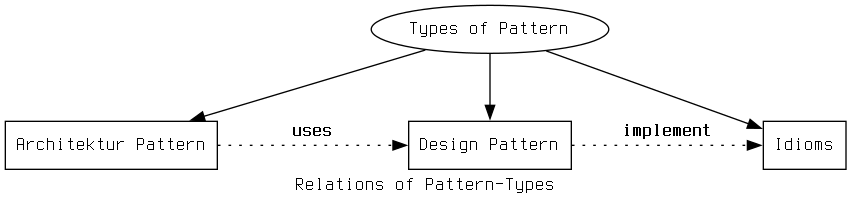
\includegraphics[width=15cm] {overview.png}
  \caption{Zusammenhang der unterschiedlichen Pattern-Typen}
  \label{overview_pattern1}
\end{center}
\end{figure}

Für meine Betrachtungen hier reicht die stark vereinfachte Sicht auf Pattern. Es gibt natürlich mehr Arten von Pattern, aber die drei in der Abbildung \ref{overview_pattern1} beschreiben sehr gut die einzelnen Schritte die notwendig sind, um ein System in einzelne Elemente zu zerlegen.

Ein Architekturmuster beschreibt die Zusammenhang zwischen einzelnen Elemente auf höherer Ebene. Klassisches Beispiel ist dabei das \textbf{\glqq Pipes-and-Filter\grqq} Pattern. Hierbei versuche ich einzelne unabhängig aggierende Elemente miteinander über defierte Pfade zu verknüpfen und nutze dabei Filter um die Informationen zu selektieren und zu filtern. Jeder kennt das Beispiel aus der Unix Welt in der einzelen Applikationen über Pipes verknüpft werden können: \textbf{\glqq ls | sort | grep | lpr\grqq}. Bei diesem Beispiel sind \textbf{sort} und auch \textbf{grep} Filter.

Dieses kann ich natürlich auch auf einer noch höheren Ebene einsetzen, z.B. besteht das Beispiel Projekt von mir aus einem Uhr-Modul und einem \textbf{externen} Audio-Modul. Da hier die beiden Module über ein Bussystem miteinander verbunden sind\footnote{ethernet}, würde aber das Patter u.a. aufgrund der Netzwerk-Kommunikation \textbf{\glqq Layers\grqq} besser passen.

Weitere interresante Architekturpattern sind \textbf{\glqq Model-View-Controller\grqq} und \textbf{\glqq Reactor\grqq}. Speziell für mein Beispiel Projekt ist der \textbf{\glqq Reactor\grqq} ein möglicher Ansatz um die Trennung des Uhr-Moduls vom eigentlich Steuerungs-Modul, welches ein Raspi-Zero Board ist, zu ermöglichen.

Ein Entwurfsmuster\footnote{Designpattern} beschreibt jetzt die Architektur einzelner Elemente auf Basis von Standart-Methoden der Realisierung. Als Beispiele kann man die ganzen \textbf{Factory Methods} nennen. Die beschäftigen sich u.a. mit der Erstellung von einzelnen Objekten

Die GoF hat die einzelen Designpattern in 3 Gruppen eingeteilt:
\begin{itemize}
  \item{Erzeugungsmuster/Creational Pattern}
  \item{Strukturmuser/Structural Pattern}
  \item{Verhaltensmuster/Behavioral Pattern}
\end{itemize}

In den weiteren Kapiteln werde ich die Patter beschreiben, die ich in meinem Beispiel Projekt benutzen werde.

Ein Idiom ist die konkrete Realisierung eines Patterns in Code. Aufgrund des Erscheinungsdatums des Buches der GoF sind nicht alle Pattern in dem Buch noch relevant. Diverse von diesen Pattern sind bereits in in C++ eingeflossen, solch eine Realisierung ist ein Idiom. Im Rahmen des Beispiel Projektes werde ich diverse Idiome erzeugen.

% Literaturverzeichnis
\begin{thebibliography} {99}
  \bibitem{gof} Erich Gamma, Richard Helm, Ralph E. Johnson, John Vlissides; Design Patterns. Elements of Reusable Object-Oriented Software; Prentice Hall; 1st ed., Reprint Edition (1. Juli 1997)
  \bibitem{grimm1} Heise Artikel C++ Blog; \url{https://www.heise.de/blog/Ein-erster-Ueberblick-Design-Patterns-und-Architekturmuster-mit-C-7147402.html} aufgerufen am 08.01.2023
\end{thebibliography}

% Index
\printindex

\end{document}
